\documentclass{article}

\usepackage{graphicx}
\usepackage{tikz}
\usepackage{tikzsymbols}
\usetikzlibrary{calc,patterns,shapes.geometric}
\pagestyle{empty}
\usepackage[margin=0pt]{geometry}
\geometry{papersize={14in,12in}}

\def\centerarc[#1](#2)(#3:#4:#5){\draw[#1] ($(#2)+({#5*cos(#3)},{#5*sin(#3)})$) arc (#3:#4:#5);}

\begin{document}
	\begin{figure}
		\centering
		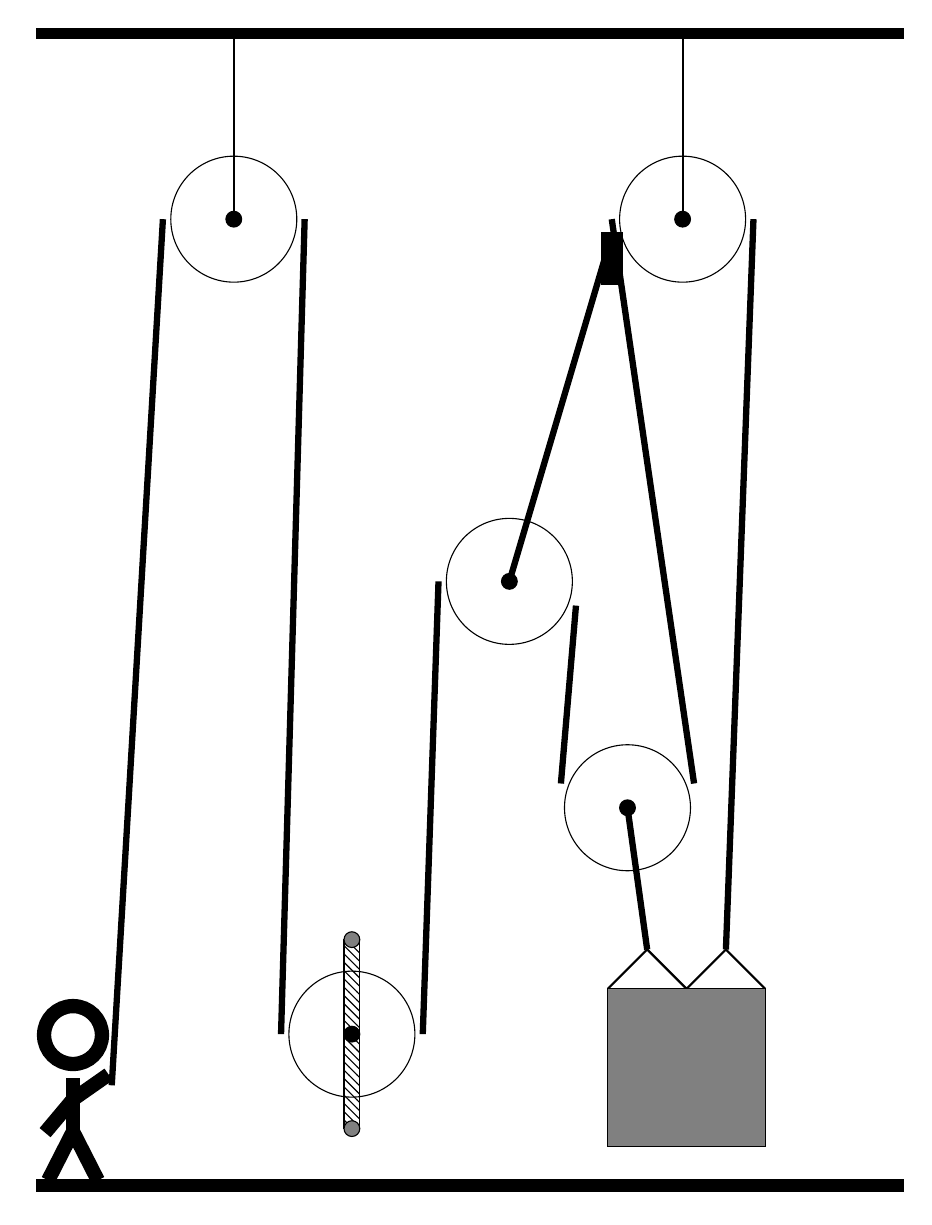
\begin{tikzpicture}
			%%%%% START %%%%%
			\draw[fill=black] (-6, 11.5) rectangle (5, 11.625);
			
			\draw (0, 4.6) circle (0.8);
			\draw[fill=black] (0, 4.6) circle (0.1);
			
			\draw (1.5, 1.725) circle (0.8);
			\draw[fill=black] (1.5, 1.725) circle (0.1);
			
			\draw (2.2, 9.2) circle (0.8);
			\draw[fill=black] (2.2, 9.2) circle (0.1);
			\draw[thick] (2.2, 9.2) -- (2.2, 11.5);
			
			\draw (-3.5, 9.2) circle (0.8);
			\draw[fill=black] (-3.5, 9.2) circle (0.1);
			\draw[thick] (-3.5, 9.2) -- (-3.5, 11.5);
			
			\draw (-2, -1.15) circle (0.8);
			\draw[fill=black] (-2, -1.15) circle (0.1);
			\draw[pattern=north west lines, pattern color=black] (-2.1, 0.05) rectangle (-1.9, -2.35);
			\draw[fill=black!50] (-2, 0.05) circle (0.1);
			\draw[fill=black!50] (-2, -2.35) circle (0.1);
			
			\draw[thick]  (1.25, -0.575) -- (1.75, -0.075) -- (2.25, -0.575) -- (2.75, -0.075) -- (3.25, -0.575);
			\draw[fill=black!50] (1.25, -0.575) rectangle (3.25, -2.575);
			\draw[line width=0.8mm] (-5.05, -1.8) -- (-4.4, 9.2);
			\centerarc[line width=0.8mm](-3.5, 9.2)(0:180:0.9);
			\draw[line width=0.8mm] (-2.6, 9.2) -- (-2.9, -1.15);
			\centerarc[line width=0.8mm](-2, -1.15)(180:360:0.9);
			\draw[line width=0.8mm] (-1.1, -1.15) -- (-0.9, 4.6);
			\draw[line width=0.8mm] (0, 4.6) -- (1.3, 9.0);
			\draw[line width=0.8mm, fill=black](1.2, 8.4) rectangle (1.4, 9.0);
			\centerarc[line width=0.8mm](0, 4.6)(-20:180:0.9);
			\draw[line width=0.8mm] (0.8457, 4.2922) -- (0.6543, 2.0328);
			
			\centerarc[line width=0.8mm](1.5, 1.725)(160:380:0.9);
			\draw[line width=0.8mm] (2.3457, 2.0328) -- (1.3, 9.2);
			\draw[line width=0.8mm](1.5, 1.725) -- (1.75, -0.075);
			\centerarc[line width=0.8mm](2.2, 9.2)(0:180:0.9);
			\draw[line width=0.8mm] (3.1, 9.2) -- (2.75, -0.075);
			
			\node at (-5.5, -1.9) {\Strichmaxerl[10][50][35]};
			
			\draw[fill=black] (-6, -3) rectangle (5, -3.15);
			%%%%% END %%%%%
		\end{tikzpicture}
	\end{figure}	
\end{document}